\documentclass[12pt,fleqn]{article}

\usepackage[utf8]{inputenc}
\usepackage[T2A]{fontenc}
\usepackage[russian]{babel}
\usepackage{graphicx}
\usepackage[footnotesize]{caption2}
\usepackage{indentfirst}
\usepackage{titlesec}

% Параметры страницы
\textheight=24cm
\textwidth=16cm
\oddsidemargin=5mm
\evensidemargin=-5mm
\marginparwidth=36pt
\topmargin=-1cm
\footnotesep=3ex
%\flushbottom
\raggedbottom
\tolerance 3000
% подавить эффект "висячих стpок"
\clubpenalty=10000
\widowpenalty=10000
\renewcommand{\baselinestretch}{1.1}
\renewcommand{\baselinestretch}{1.5} %для печати с большим интервалом
\newcommand{\sectionbreak}{\clearpage}
\renewcommand{\labelenumii}{\arabic{enumi}.\arabic{enumii}.}



\begin{document}
\sloppy
	
\begin{titlepage}
\newpage
		
\begin{figure}[t]
	\centering
	
\includegraphics[width=0.4\textwidth]{img/mgu}
\end{figure}
		
\begin{center}
Московский государственный университет имени М.В. Ломоносова \\
Факультет вычислительной математики и кибернетики \\
Кафедра автоматизации вычислительных комплексов \\
\end{center}
		
\vspace{6em}
\begin{center}
\large
Ермакова Татьяна Ивановна
\end{center}
		
\begin{center}
\Large
\bfseries
Метод и средства передачи данных в реальном времени в программно-конфигурируемых сетях
\end{center}

\begin{center}
\large
\textsc{
	выпускная квалификационная работа
}
\end{center}

\vspace{4em}
\begin{flushright}
	\textbf{Научный руководитель:}\\
	к.ф.-м.н с.н.с\\
	В.В.Балашов\\
\end{flushright}%


\vspace{\fill}
\begin{center}
Москва 2019
\end{center}
		
\end{titlepage}


\renewcommand{\contentsname}{Содержание}
\tableofcontents

\section*{Введение}
\addcontentsline{toc}{section}{Введение}
текст

\section{Постановка задачи}
Целью работы является разработка подхода к использованию программно-конфигурируемых сетей в составе вычислительных реального времени. В основу подхода положена ранее разработанная автором схема управления потоками данных в ПКС на основе виртуальных каналов. Для достижения этой цели должны быть решены следующие задачи:
\begin{enumerate}
	\item Разработка алгоритма динамической реконфигурации виртуальных каналов.
	\item Реализация приложения для контроллера ПКС, выполняющего функции мониторинга сети и её реконфигурации при выявлении отказов.
	\item Экспериментальное исследование полученного решения по критерию работоспособности в условиях реального времени.
\end{enumerate}

\section{Управление трафиком в ВС реального времени с использованием виртуальных каналов} \label{sec:scheme}
\subsection{Схема управления трафиком}
\subsection{Реализации схемы управления трафиком}
\subsection{Сравнение реализаций по критерию поддержки реконфигурируемости}
Конфигурацией сети на основе виртуальных каналов назовем набор параметров виртуальных каналов в совокупности с их маршрутами. Каждой конфигурации соответствует набор таблиц маршрутизации, определяющих действия коммутаторов по передаче данных и контролю трафика в соответствии с данной конфигурацией.

Стандарт AFDX предусматривает наличие одной фиксированной таблицы маршрутизации на каждом коммутаторе. Такой набор таблиц маршрутизации соответствует единственной доступной в сети AFDX конфигурации.

Стандарт FC-AE-ASM-RT имеет возможность поддерживать на коммутаторах несколько таблиц маршрутизации, задаваемых до начала работы ы. Это позволяет задать несколько конфигураций сети. Переход между такими конфигурациями осуществляется при помощи контроллера конфигураций. Им является дополнительная оконечная станция. При смене конфигурации контроллер сообщает коммутаторам сети идентификатор новой конфигурации. На каждом коммутаторе находится внутренняя оконечная станция, обрабатывающая информацию о смене конфигурации. Так как контроллером передается только идентификатор, весь набор конфигураций должен быть заложен в коммутаторы до начала работы ы.

В ПКС таблицы коммутаторов управляются контроллером при помощи сообщений, регламентируемых протоколом OpenFlow. В предложенной автором схеме модификация параметров виртуальных каналов производится сообщениями FlowMod и MeterMod протокола OpenFlow1.3. За счёт этого таблицы маршрутизации, равно как и meter-таблицы, могут быть изменены любым образом в ходе работы ы. Это позволяет создавать множество конфигураций, размер которого ограничен лишь возможностями физической среды передачи данных.

Динамическая реконфигурация сетей ВСРВ требуется в случаях:
\begin{enumerate}
	\item смены режимов работы;
	\item выхода из строя вычислителей.
\end{enumerate}

Как было показано выше стандарт AFDX не поддерживает реконфигурацию в ходе работы ы. Возможностей же FC-AE-ASM-RT недостаточно для произведения гибкой реконфигурации, так как все сбойные режимы должны быть заранее заложены в у. Для единичного отказа число таких режимов является достаточно большим и оценивается количеством физических элементов сети. Расчет всех случаев множественного отказа является ещё более нетривиальной задачей, а хранение всех таких конфигураций в памяти коммутаторов не представляется возможным. Использование ПКС в ВС РВ позволяет производить расчет и применение новой конфигурации сети непосредственно при возникновении поломки. Это даёт возможность гибко реагировать на множественные сбои и восстанавливать работу ы в полном объеме в тех случаях, когда это позволяют физические ресурсы.


\section{Актуальность задачи}
Динамическая реконфигурация сети востребована в ВС РВ. Возможность перераспределить потоки данных в ходе работы ы необходима при возникновении сбоев или желании заложить несколько режимов работы в у.

В разделе \ref{sec:scheme} было продемонстрировано, что в ПКС имеются возможности для гибкой реконфигурации сети при соблюдении требований к качеству обслуживания, принятых в сетях ВС РВ. Для осуществления реконфигурации в случае возникновения сбоев необходимо:
\begin{enumerate}
	\item Определить, в какой части сети произошел сбой.
	\item Произвести расчет новой конфигурации с учетом вышедших из строя элементов сети.
	\item Произвести переход на полученную конфигурацию.
\end{enumerate}

Данная работа посвящена вопросу идентификации сбоев и алгоритму расчета новой конфигурации сети. Процедура смены конфигураций была ранее реализована и апробирована автором на предмет пригодности в рамках подтверждения работоспособности схемы управления трафиком в ПКС.

\section{Алгоритм реконфигурации виртуальных каналов}
\subsection{Общая схема алгоритма}
\subsection{Процедуры поиска нового маршрута виртуального канала}
\subsection{Описание базового этапа алгоритма}
\subsection{Описание дополнительного этапа алгоритма}


\section{Структура и функции приложения реконфигурации}
\subsection{Структура приложения реконфигурации}
\subsection{Описание функций служебной части}
\subsection{Описание функций управляющей части}
\subsection{Описание функций монитора}


\section{Программная реализация}
\subsection{Выбор базового программного обеспечения сети}
\subsection{Структура программного средства}
текст


\section{Экспериментальное исследование}
\subsection{Цель исследования}
Целью исследования является подтверждение характеристик предложенного в работе алгоритма реконфигурации виртуальных каналов, предназначенного для использования в рамках описанного подхода к передаче данных в ПКС в условиях реального времени. Для достижения поставленной цели необходимо:
\begin{itemize}
	\item провести исследование свойств алгоритма на различных классах входных данных; 
	\item провести апробацию работы алгоритма в составе приложения, реализующего функции реконфигурации и мониторинга.
\end{itemize}

Свойства алгоритма, подлежащие исследованию:
\begin{itemize}
	\item успешность и этап завершения;
	\item скорость работы.
\end{itemize}

Изучаемые в рамках апробации подхода характеристики ы:
\begin{itemize}
	\item успешность восстановления трафика в сети после завершения работы алгоритма реконфигурации;
	\item скорость применения изменений в сети;
	\item характеристики качества обслуживания для трафика абонентов (задержка и джиттер).
\end{itemize}

\subsection{Классы исходных данных}
Параметры для формирования классов данных:
\begin{enumerate}
	\item Распределение каналов по пропускным способностям.
	\item Общая загруженность сети.
	\item Топология сети.
\end{enumerate}

Расчёт пропускной способности виртуального канала производится в соответствии с формулой:
$$bw = \frac{LM}{BAG}$$

Выделим типы виртуальных каналов в зависимости от пропускной способности:
\begin{itemize}
	\item легковесные ($bw=k$);
	\item средние ($bw=2k$);
	\item тяжёлые ($bw=4k$).
\end{itemize}

Классы исходных данных, сформированные на основе процентного содержания виртуальных каналов каждого типа, показаны в таблице~\ref{table:bwclass}. Данные классы выбраны для исследования случаев преобладания каждого из типов виртуальных каналов. Распределение пропускных способностей входных потоков данных влияет на работу алгоритма, так как поиск альтернативного маршрута виртуальных каналов затрудняется с ростом их пропускной способности.

\begin{table}[h]
\begin{center}
\begin{tabular}{|c|c|c|c|}
\hline
	 & Легковесные & Средние & Тяжёлые\\
\hline
	1 & 90\% & 7\% & 3\% \\
\hline
 2 & 10\% & 80\% & 10\% \\
\hline
	3 & 33\% & 34\% & 33\% \\
\hline
	4 & 5\% & 15\% & 80\% \\
\hline
\end{tabular}
\end{center}
\caption{Классы данных на основе пропускной способности}
\label{table:bwclass}
\end{table}

Расчёт общей загруженности сети производится при помощи формулы, отражающей утилизацию физических линий в зависимости от количества маршрутов виртуальных каналов, которые могут быть проложены через данную линию.

Для графа сети, в котором ребра соответствуют физическим линиям, введём вес ребра $e$:
$$p_{e} = \sum_{vl}\frac{bw_{vl} \ast k_{vl_e}}{k_{vl}}$$
где 
\begin{itemize}
	\item $vl$ -- множество виртуальных каналов;
	\item $bw_{vl}$ -- пропускная способность виртуального канала;
	\item $k_{vl_e}$ -- число кратчайших путей, построенных для данного канала, проходящих через это ребро;
	\item $k_{vl}$ -- количество найденных кратчайших путей для данного виртуального канала.
\end{itemize}

Тогда общая загруженность сети определяется формулой:
$$p = \max_{e}\frac{p_{e}}{bw_{e}}$$

где $bw_{e}$ -- пропускная способность физической линии.

Два класса исходных данных, формирующиеся на основе данного параметра, показаны в таблице~\ref{table:loadclass}. Общая загруженность сети влияет на работу исследуемого алгоритма. С ростом загруженности возрастает сложность поиска альтернативных маршрутов для виртуальных каналов. 

\begin{table}[h]
\begin{center}
\begin{tabular}{|c|c|}
\hline
	& Загруженность сети ($p$)\\
\hline
	1 & 60\% \\
\hline
	2 & 80\% \\
\hline
\end{tabular}
\end{center}
\caption{Классы данных на основе загруженности сети}
\label{table:loadclass}`
\end{table}

Для апробации выхода из строя различных элементов сети и демонстрации множества вариантов поиска альтернативного маршрута было выбрано три топологии:
\begin{enumerate}
	\item <<Ромб>> (Рис.~\ref{pic:4node}).
	\item <<Двойное резервирование>> (Рис.~\ref{pic:double}).
	\item <<add Название>> (Рис.~\ref{pic:5node}).
\end{enumerate}

\begin{figure}[h!]
	\centering
	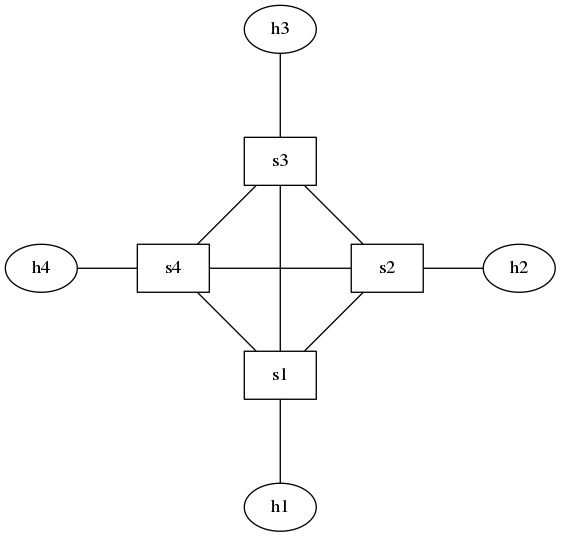
\includegraphics[width=0.40\textwidth]{img/4node.png}
	\caption{Топология <<Ромб>>.}
	\label{pic:4node}
\end{figure}

\begin{figure}[h!]
	\centering
	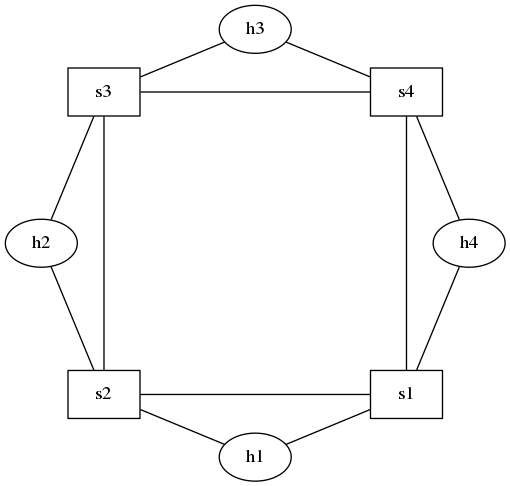
\includegraphics[width=0.40\textwidth]{img/double.png}
	\caption[russian]{Топология <<Двойное резервирование>>.}
	\label{pic:double}
\end{figure}

\begin{figure}[h!]
	\centering
	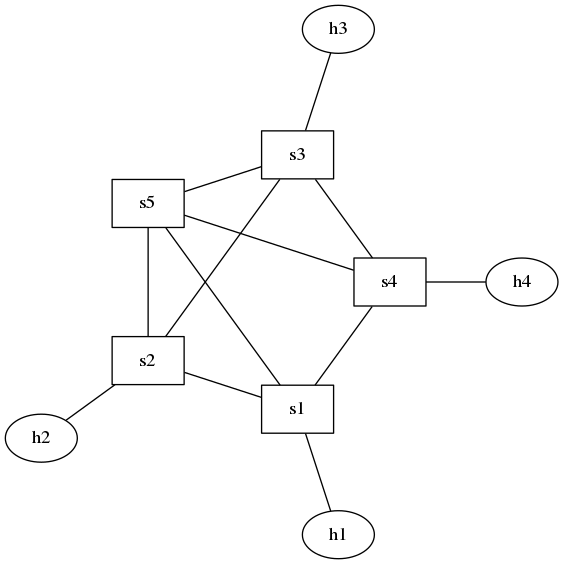
\includegraphics[width=0.40\textwidth]{img/5node.png}
	\caption{Топология <<add Название>>.}
	\label{pic:5node}
\end{figure}

В исследовании используется рекомендованное экспертами в области вычислительных реального времени число потоков данных равное 100.

\subsection{Исследование свойств алгоритма}
\subsubsection{Методика исследования}
Исследование свойств алгоритма производится по следующей схеме:
\begin{enumerate}
	\item Для каждого класса данных генерируется соответствующий ему набор виртуальных каналов.
	\item Для каждого набора виртуальных каналов:
	\begin{enumerate}
		\item Запускается приложение, содержащее алгоритм реконфигурации.
		\item Запуск инициирует построение начальных маршрутов виртуальных каналов.
		\item Собирается статистика по количеству виртуальных каналов, проходящих через каждый элемент сети.
		\item Выбирается элемент сети, через который проходит наибольшее число виртуальных каналов, и имитируется его поломка.
		\item Поломка инициирует запуск алгоритма реконфигурации.
		\item По завершению алгоритм выдаёт информацию об успешности и этапе завершения, а так же времени работы.
	\end{enumerate}
	\item add Метрика для сравнения времени работы алгоритма с чем-то.
	\item По полученным характеристикам делается вывод о возможности использования алгоритма в рамках подхода к передаче данных в реальном времени.
\end{enumerate}
 
\subsubsection{Результаты}
Характеристики компьютера, на котором производилось исследование:
\begin{itemize}
	\item Процессор -- Intel Core i7, тактовая частота 1.90 ГГц.
	\item Оперативная память -- 4 ГБ.
\end{itemize}

Результаты исследования свойств алгоритма реконфигурации виртуальных каналов приведены в addПриложение (см. таблицу addТаблица).

Максимальное время работы алгоритма – addмс. Данные показатели времени достигаются, если алгоритм вынужден выполнить дополнительный этап. Следует отметить, что выполнение дополнительного этапа произошло в add\% случаев. Как правило алгоритм завершает работу на базовом этапе. При таком варианте выполнения время завершения алгоритма не превышает addмс.

Алгоритм не смог построить новую у виртуальных каналов при add. Это объясняется тем, что add.

add Возможно стоит сказать что-то о соотношении времени работы алгоритма и задержек в сети чтобы знать почему это нормально. Может типовые периоды сообщений?

\subsection{Апробация разработанного подхода динамической реконфигурации сети}
\subsubsection{Конфигурация экспериментальной ы}
 а апробации представляет собой виртуальную среду, имитирующую
функционирование:
\begin{enumerate}
	\item Контроллера сети.
	\item Набора коммутаторов.
	\item Абонентов сети, формирующих потоки данных с заданными характеристиками.
\end{enumerate}

Виртуальная среда разворачивается на основе операционной ы Ubuntu 16.04,
на которой установлены следующие компоненты:
\begin{enumerate}
	\item Runos -- ПКС-контроллер [addlink].
	\item Ofsoftswitch13 -- программный коммутатор, поддерживающий OpenFlow 1.3 [addlink].
	\item Mininet -- средство имитирующее работу сети [addlink].
\end{enumerate}

\subsubsection{Сценарии апробации}

Для апробации предложенного подхода к передаче данных в реальном времени был выбран набор сценариев, основывающийся на том, какие элементы сети могут выйти из строя. 

Рассматривается выход из строя:
\begin{enumerate}
	\item Коммутатора.
	\item Физической линии, соединяющей два коммутатора.
	\item Физической линии, соединяющей абонента с коммутатором.
	\item Порта абонента или коммутатора.
\end{enumerate}

Дополнительно к этому рассматриваются сценарии кратных последовательных во времени выходов из строя элементов сети.

Сценарии разрыва физической линии между коммутаторами и выхода из строя соответствующих портов производятся на всех топологиях. Оставшиеся сценарии могут быть выполнены только на топологиях <<Двойное резервирование>> и <<add Название>> (см. Рис.~\ref{pic:double} и Рис.~\ref{pic:5node}).

\subsubsection{Методика апробации}
Апробация работы алгоритма реконфигурации в рамках предложенного подхода состоит из трёх этапов:
\begin{enumerate}
	\item Формирование набора тестовых прецедентов.
	\item Проведение экспериментов на тестовых прецедентах.
	\item Анализ результатов.
\end{enumerate}

Тестовые прецеденты формируются выбором:
\begin{itemize}
	\item сценария апробации;
	\item класса исходных данных с доступной для выбранного сценария топологией сети.
\end{itemize}

На этапе проведения экспериментов производится запуск каждого тестового прецедента:
\begin{enumerate}
	\item Формируется соответствующая классу данных конфигурация сети.
	\item Запускается приложение реконфигурации.
	\item Запускается виртуальная тестовая среда, имитирующая поведение сети.
	\item Запуск приложения инициирует построение начальных маршрутов виртуальных каналов.
	\item Запуск тестовой среды инициирует отправку и прием потоков данных абонентами, а так же сбор статистики по этим потокам данных.
	\item Средствами тестовой среды запускается сценарий апробации.
	\item Соответствующая сценарию поломка инициирует запуск алгоритма реконфигурации.
	\item По завершению алгоритм выдаёт информацию о времени, затраченном на применение изменений в сети.
	\item Происходит сворачивание тестовой среды, инициирующее обработку собранной статистики по потокам данных.
\end{enumerate}

На этапе анализа результатов для каждого тестового прецедента:
\begin{enumerate}
	\item Проверяется факт восстановления трафика по завершению выполнения сценария.
	\item Анализируется время, затраченное на применение изменений в сети. add как
	\item Анализируется число потерянных в ходе реконфигурации пакетов. add как
	\item Задержки и джиттеры, полученные в период реконфигурации сравниваются с эталонными задержками, полученными в штатном режиме.
	\item Делается вывод об успешности работы приложения реконфигурации в рамках предложенного сценария.
\end{enumerate}

\subsubsection{Результаты}

Результаты апробации работы алгоритма в рамках приложения, реализующего подход к передаче данных в условиях реального времени в ПКС, приведены в addПриложение (см. таблицу addТаблица).

Джиттеры и задержки потоков данных, виртуальные каналы которых участвовали в реконфигурации, отличались от эталонных не более, чем на addмс и addмс соответственно. Данное отклонение лежит в рамках допустимого.

Потери пакетов составили add сколько + метрика. add вывод из этого.

Отказы от построения новых виртуальных каналов были получены на тех же классах данных, что и при исследовании свойств алгоритма.

Было проверено несколько сценариев кратного последовательного во времени выхода из строя элементов сети. Максимальное число последовательных поломок, после которых восстанавливалась работоспособность ы, составило add. Отказы от восстановления работы сети после очередной поломки были обусловлены исключительно отсутствием путей между абонентами или нехваткой пропускных способностей.

\subsection{Выводы}
Проведенное экспериментальное исследование продемонстрировало, что:
\begin{itemize}
	\item основные характеристики алгоритма соответствуют ожидаемым;
	\item алгоритм успешно функционирует в рамках приложения реконфигурации, работающего в виртуальной среде, имитирующей сеть ПКС;
	\item соблюдаются ограничения на характеристики качества обслуживания абонентских потоков данных при реконфигурации сети с использованием предложенного алгоритма.
\end{itemize}

Исследование и апробация показали, что предложенный алгоритм реконфигурации виртуальных каналов способен работать в составе приложения, реализующего подход к передаче данных в реальном времени в ПКС. Алгоритм успешно и за приемлемые промежутки времени осуществляет поиск новых маршрутов для виртуальных каналов при выходе из строя различных элементов сети. Апробация показала работоспособность разработанного приложения, осуществляющего функции реконфигурации и мониторинга, и реализуемого им подхода. 

\section*{Заключение}
\addcontentsline{toc}{section}{Заключение}
текст

\renewcommand{\bibname}{Список литературы}

\end{document}